\documentclass[12pt]{article}

\usepackage{sbc-template}
\usepackage{graphicx,url}
\usepackage[utf8]{inputenc}
\usepackage[brazil]{babel}

     
\sloppy

\title{Identificando Linhas de Códigos Comentadas em Repositórios de Software}

\author{Vitor Botelho Vaz de Melo\inst{1}, André Hora\inst{1} }


\address{Departamento de Ciência da Computação -- Universidade Federal de Minas Gerais
  (UFMG)\\
  Belo Horizonte -- MG -- Brazil
  \email{\{vitormelo,andrehora\}@dcc.ufmg.br}
}

\begin{document} 

\maketitle

\begin{abstract}
  This paper describes the training of a classifier for identification
  of commented-out code in several source codes from different free software 
  repositories. Commenting-out code is a bad programming practice and can cause 
  problems such as decreased readability, loss of productivity, among others. Identify
  this practice will allow us to better understand how it is present in the 
  software development.
\end{abstract}
     
\begin{resumo} 
  Este trabalho descreve o treinamento de um classificador para a identificação 
  de código removido por comentário (\textit{commented-out code}) em diversos 
  códigos fontes de diferentes repositórios de software livre. Remover código 
  através de comentários é uma má prática de programação e pode causar problemas 
  como diminuição da legibilidade, perda de produtividade, entre outros. Identificar
  esta prática nos permitirá entender melhor como ela esta presente no desenvolvimento
  de software.
\end{resumo}


\section{Introdução} \label{sec:intr}

À medida que a Ciência da Computação avança e milhões de linhas de códigos são 
escritas, diariamente e em diversas linguagens de programação, os desenvolvedores 
percebem que, para alcançar sucesso a médio e longo prazo em seus projetos, é
necessário utilizar-se, cada vez mais, das melhores ferramentas e práticas de 
programação. 

Uma prática de programação muito comum ao se desenvolver softwares é a de 
''remover'' uma linha ou um bloco de código tornando-os comentários, sendo conhecida  
como commented-out code (Figura \ref{fig:commentExample}). Comentar uma linha de código 
pode ser útil, tanto que 
os próprios ambientes de programação (IDE's e editores de texto) oferecem atalhos 
fáceis para isso. Contudo, esta prática se torna um verdadeiro problema quando 
estes códigos comentados estão inseridos em um sistema grande, complexo e
mantido por diversas pessoas \cite{cleanCode}.

\begin{figure}[ht]
  \centering
  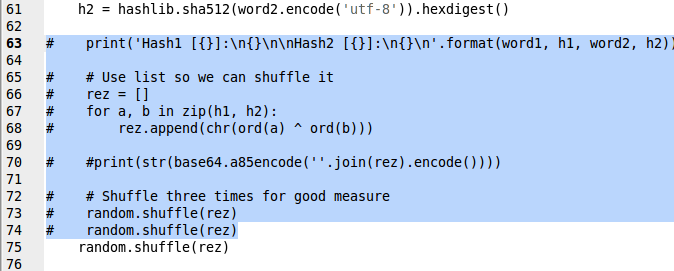
\includegraphics[width=0.9\textwidth]{../images/gcc06.png}
  \caption{Commented-out code example }
  \label{fig:commentExample}
\end{figure}


A inserção de código comentado nos arquivos fontes de um sistema pode causar
redução da legibilidade, distração e perda de tempo. Martin, em seu livro clássico
Clean Code, enfatiza \textit{Few practices are as odious as commenting-out code. 
Don’t do this!}, ele argumenta que outras pessoas não terão coragem de deletar 
este código por achar que ele pode ser importante~\cite{cleanCode}. 

Além disso, quando um mantenedor se depara com códigos comentados ele pode ter uma 
série de dúvidas, como \textit{"Por que este código está comentado? Isso é útil em 
alguma função? Este código está relacionado com determinada mudança?"}, entre outras 
questões específicas para cada sistema. Este tipo de reflexão pode no mínimo ser 
uma perda de tempo, ou até mesmo uma distração para introduzir bugs no sistema \cite{cleanCode}.

Este trabalho tem como principal objetivo fazer um estudo abrangente desta prática em repositórios 
de código aberto. No entanto, existem poucos estudos científicos abordando esta problemática e não 
há, entre as ferramentas mais populares, uma solução que identifica automaticamente
este tipo de comentário \cite{articleMiningComments}. Portanto, este trabalho descreve o
desenvolvimento de uma ferramenta apropriada utilizando técnicas de aprendizado de 
máquina. Em trabalhos futuros essa ferramenta será utilizada para analisar diversos
repositórios de software de código aberto. 

\section{Trabalhos Anteriores} \label{sec:prev-works}
GRIJÓ L. e HORA A. exploraram o problema da inserção de \textit{commented-out code}
e demonstraram seus interessantes resultados no artigo Minerando Código Comentado 
\cite{articleMiningComments}. No trabalho foi desenvolvido um parser heurístico
que identifica \textit{commented-out code} para a linguagem java que obteve
uma precisão de 83\%. Com esta ferramenta foi identificado que alguns 
sistemas possuem como mediana 4,17\% de taxa de commented-out code em relação
ao total de comentários, com alguns sistemas chegando a 30\%.

Este trabalho propõe uma extensão ou continuação desse estudo, a fim de validar
e aprofundar o conhecimento sobre os resultados obtidos. Para isso, a primeira etapa foi 
desenvolver uma ferramenta com maior precisão na identificação de 
\textit{commented-out code} e que seja multi linguagem.  

\section{Modelo de Identificação de \textit{Commented-out Code}}

Separar o que é código removido por comentário do que é comentário real, não é
uma tarefa fácil. Se considerarmos ferramentas como parsers de linguagem ou
mesmo expressões regulares, o identificador pode sofrer com algumas situações, como:
\begin{itemize}
  \item[1] Códigos não finalizados
  \item[2] Códigos velhos e que não compila mais
  \item[3] Código misturado com textos, etc. 
\end{itemize}

Além disso, essas ferramentas teriam que ser implementadas considerando uma linguagem
alvo, requerindo um esforço muito alto de desenvolvimento de software para fazer um 
estudo multi-linguagem, consequentemente impossibilitando este estudo acadêmico. Por 
outro lado, modelos de classificação podem aprender a separar as linhas de código de 
comentários a partir de exemplos~\cite{patternClassification}. E esses exemplos temos 
disponíveis em grande quantidade nos repositórios de código livre em ferramentas como 
o github\footnote{https://github.com/}.

\subsection{Definição do Modelo de Classificação}

Para realizar a tarefa de classificação foi utilizado uma rede neuronal profunda com
a arquitetura LSTM (Long short-term memory)~\cite{gers1999learning} (Figura ~\ref{fig:simple-model}). 
Essa é uma rede neural recorrente, o que permite criar uma estrutura ''temporal'' de recebimento da 
entrada.

A entrada do modelo definido é o equivalente a uma linha de um código fonte, considerando
que essa linha pode ser um comentário ou código. O modelo recebe essa linha caractere por 
caractere. A intuição por tras dessa escolha está no fato de que o código utiliza mais de
caracteres especiais como '\{', '\}', '(', ')', '=', entre outros. Além disso, a 
arquitetura recorrente permite que a rede aprenda as estruturas sequenciais que os caracteres
podem formar, como por exemplo a chamada de uma função: ''f(x)''.

O modelo conta ainda com uma camada de embedding que permite o aprendizado de uma representação
distribuída dos caracteres~\cite{mikolov2013distributed}. Dessa forma os caracteres podem ter uma
certa semântica ou peso para o modelo, facilitando o aprendizado como um todo. E ao final temos
uma camada totalmente conectada e a camada de saída, com função de ativação sigmoid~\cite{zurada1992introduction}.

\begin{figure}[ht]
  \centering
  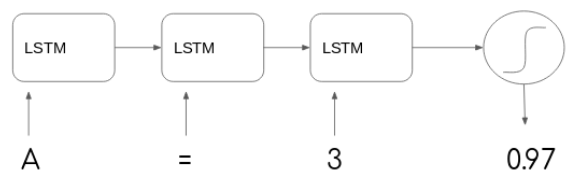
\includegraphics[width=0.6\textwidth]{../images/simple-model.png}
  \caption{ Arquitetura do modelo simplificada - no modelo desenvolvido cada 
  caractere é recebido como entrada por uma LSTM de forma sequencial, ao final
  obtemos uma saída com a função de ativação sigmoid em que o resultado é uma 
  predição para a linha de código entre 0 e 1, no qual consideramos que quanto
  mais próximo de 1, maior a probabilidade da linha ser realmente código}
  \label{fig:simple-model}
\end{figure}

\section{Obtenção e pré-processamento dos dados} \label{sec:dev}

Antes de treinar o modelo foi necessário a construção de uma base de dados de
treino. Para a constituição da base foram realizadas as atividades descritas 
nas seções seguintes.

\subsection{Download de Repositórios de Software}
A primeira etapa foi realizar o download do código fonte de diversos repositórios.
Para isso foi utilizado a api do github para escolher os repositórios de
código aberto com uma boa evolução, que seja ativo, e de forma a construir uma base
com uma variabilidade de estilo de código, e linguagem. 
Isso se traduziu nos seguintes critérios adotados para fazer o download dos dados:
\begin{itemize}
  \item Pegar os 10 primeiros repositórios mais populares por
  linguagem de  programação ( com mais estrelas)
  \item O primeiro commit deve ter mais de 2 anos
  \item O último commit deve ter menos de 1 mês
\end{itemize} 

As linguagens utilizadas foram C, Java, Javascript e
Typescript.

\subsection{Separação de comentários e código}

Nesta etapa pré processamos todos os arquivos fontes e os separamos em dois arquivos. 
Um arquivo restando somente linhas de código e outro somente comentários.
Foi utilizado uma expressão regular para fazer essa separação (Figura \ref{fig:regex}).

\begin{figure}[ht]
  \centering
  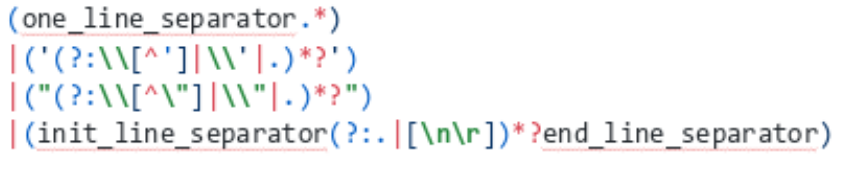
\includegraphics[width=0.6\textwidth]{../images/regex.png}
  \caption{Expressão regular utilizada para separar código fonte em comentários e código.
  Este regex tem três partes principais, a primeira identifica os comentários de uma linha,
  a segunda exclui os possíveis casos de uso do indicador de comentário dentro de uma string,
  e a terceira identifica os comentários de bloco }
  \label{fig:regex}
\end{figure}

Na Figura \ref{fig:sep-comment} podemos observar um exemplo deste processamento.
Repare que neste momento ainda não identificamos os códigos removidos por comentário. 

\begin{figure}[ht]
  \centering
  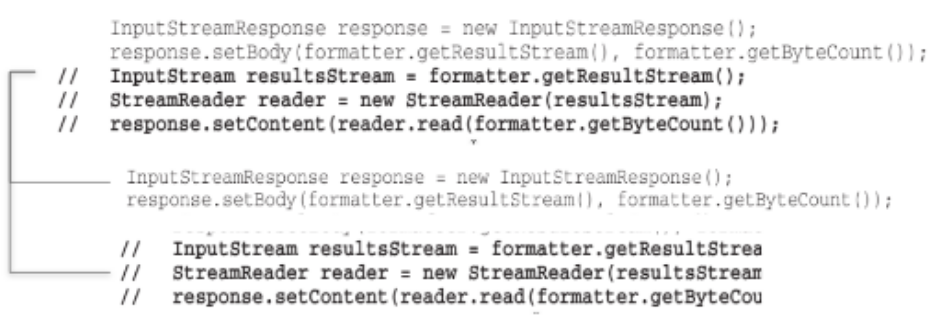
\includegraphics[width=0.8\textwidth]{../images/separated-comments.png}
  \caption{Exemplo de código fonte separado em duas partes (código e comentários) }
  \label{fig:sep-comment}
\end{figure}


\subsection{Definição dos dados de treino}
 
Após a separação em código e comentário foi definido o modelo final para os dados de treino,
no qual para cada linha temos se é um comentário '0' ou código '1' (Tabela \ref{tab:amostra-dados}). Além disso, foi filtrado
linhas com menos de 3 caracteres, ou vazias. Dessa forma evitamos muitas linhas que são só 
abertura ou fechamento de escopo, entre outras.

\begin{table}[ht]
  \centering
  \caption{Amostra dos dados de treino final}
  \label{tab:amostra-dados}
  \begin{tabular}{llr}
    Language & Line & Is Code\\[0.5ex]
    \hline
    Javascript	& return output; &	1.0\\[0.5ex]
    C++ &	if (visitable(sub)) \{ &	1.0\\[0.5ex]
	  C	& loss of use, data, or profits; or business i... &	0.0\\[0.5ex]
    \hline
  \end{tabular}
\end{table}

Temos ao final, portanto, uma base que usa diversas linhas de código, e diversos comentários
reais. Dessa forma, o objetivo de nosso modelo vai ser simplesmente aprender o que é código e
o que é um comentário, identificar os \textit{commented-out code} será um passo secundário. 

A base de treino ficou com cerca de 12 milhões de linhas de código, com 19,5\% sendo comentário 
e 80,5\% código. Além disso, temos a seguinte proporção de linhas por linguagem.

\begin{table}[ht]
  \centering
  \caption{Proporção da base de dados por linguagem}
  \label{tab:prop}
  \begin{tabular}{lr}
    Language & (\%) \\[0.5ex]
    \hline
    Java & 25.4 \\[0.5ex]
    Javascript	& 24.5 \\[0.5ex]
    Typescript & 18.0 \\[0.5ex]
    C	& 23.4 \\[0.5ex]
    C++ &	3.0 \\[0.5ex]
    \hline
  \end{tabular}
\end{table}

E para cada linguagem temos a proporção de comentários e de código.

\begin{table}[ht]
  \centering
  \caption{Proporção de comentários e código por linguagem}
  \label{tab:prop2}
  \begin{tabular}{lrr}
    Language & Código (\%) & Comentário (\%)\\[0.5ex]
    \hline
    Java & 79.4 & 20.6 \\[0.5ex]
    Javascript & 83.0	& 17.0 \\[0.5ex]
    Typescript & 70.8 & 29.2 \\[0.5ex]
    C	& 86.9 & 13.1 \\[0.5ex]
    C++ & 79.2 &	20.8 \\[0.5ex]
    \hline
  \end{tabular}
\end{table}

\section{Treinamento e Avaliação}

Nesta etapa os dados foram separados aleatoriamente em dados de treino (80\%)
e em dados de teste (20\%). Após o treino durante 30 épocas, o modelo obteve uma
acurácia de 98\% tanto para os dados de treino quanto para os dados de teste.

Na figura \ref{fig:tresh} podemos observar como o modelo se comporta para diferentes
níveis de treshold da saída. A ROC é quase perfeita, mostrando que o modelo separa 
muito bem os códigos e comentários. Podemos observar também a acurácia, a precisão
e a revocação para alguns tresholds. Para o modelo final foi escolhido o treshold em 0.6,
pois mantém a melhor acurácia e maior precisão.

\begin{figure}[ht]
  \centering
  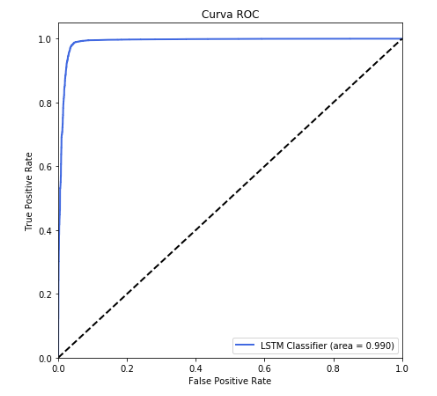
\includegraphics[width=0.45\textwidth]{../images/roc06.png}
  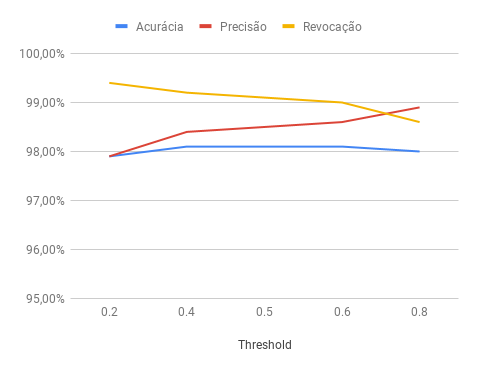
\includegraphics[width=0.45\textwidth]{../images/chart-tresh.png}
  \caption{Acurácia, Precisão e Revocação para diferentes tresholds na saída 
  e Curva ROC (Receiver Operator Curve) }
  \label{fig:tresh}
\end{figure}


\begin{figure}[ht]
  \centering
  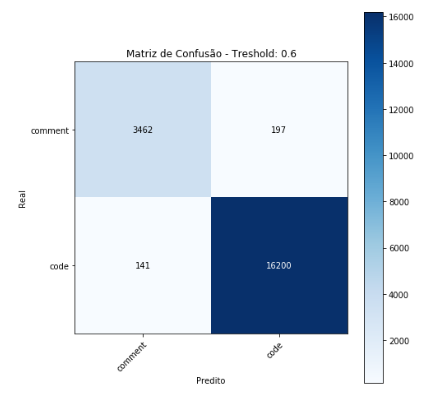
\includegraphics[width=0.45\textwidth]{../images/confmat.png}
  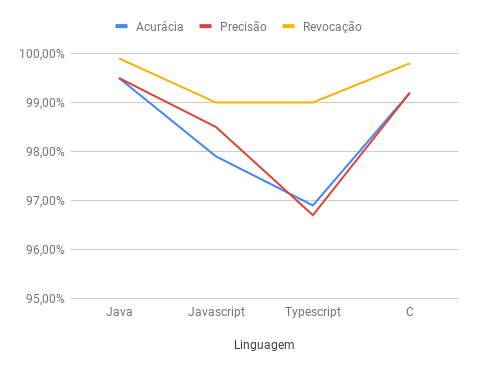
\includegraphics[width=0.45\textwidth]{../images/chart-ling.png}
  \caption{Matriz de confusão e estatísticas para as diferentes linguages }
  \label{fig:confmat}
\end{figure}


Já com o treshold definido em 0.6 podemos observar na figura \ref{fig:confmat} a  matriz de 
confusão, com os valores detalhados predição para uma amostra de trinta mil dados de teste.
Em sequência podemos observar a acurácia, precisão e revocação para as diferentes linguagens,
a linguagem Typescript se destaca com relação às outras, com uma acurácia e precisão mais próximas
de 97\%, porém esse valor faz sentido uma vez que essa linguagem tem uma proporção maior de 
comentários (Tabela \ref{tab:prop2}). Além disso, o modelo erra mais comentários, classificando
cerca de 5.6\% dos comentários como código.


No entanto, quando olhamos para esses erros (Tabela \ref{tab:commentout}) encontramos os 
\textit{commented-out code}. Mostrando mais uma vez que o modelo foi capaz de aprender o 
que é código, e agora podemos separar estes ''ruídos'' dos comentários. Além disso, a taxa 
de erro de 5.6\% é uma boa aproximação da taxa de \textit{commented-out code} nessa base, se
aproximando da mediana de 4.17\% encontrado por \cite{articleMiningComments}. 
\begin{table}[ht]
  \centering
  \caption{Linhas consideradas comentários na base de dados que o modelo classificou como código}
  \label{tab:commentout}
  \begin{tabular}{lrr}
    Line & Is code & Predito\\[0.5ex]
    \hline
    system.out.println(sw.gettotaltimemillis()); & 0.0 & 0.981\\[0.5ex]
    mydomainclass myobject = unmarshaller.unmarshal(source); & 0.0	& 0.995 \\[0.5ex]
    public jmshandlermethodfactory myjmshandlermethodfactory()  & 0.0 & 0.998 \\[0.5ex]
    \hline
  \end{tabular}
\end{table}



\section{Considerações Finais}

O modelo proposto se mostrou robusto e preciso durante a fase de avaliação. 
Com ele será possível entender a fundo a prática de remover código através
de comentários em diferentes repositórios de software de direntes linguanges.
O classificador ainda pode ser evoluído treinando-o com mais linguagens. 
E novas avalições podem ser interessantes, como testar o modelo em códigos 
de uma linguagem de programação em que ele não foi treinado.

\bibliographystyle{sbc}
\bibliography{references}

\end{document}
